\documentclass{article}
\usepackage{graphicx}
\usepackage{url}
%\usepackage{hyperref}
\usepackage{verbatim}
%\usepackage{times,mathptm}
\usepackage{times}
% the following package is optional:
%\usepackage{latexsym}
%\usepackage{picins}
\usepackage{url}
\usepackage{epsfig}
\usepackage{amsmath}
%\usepackage{macros}
%\usepackage{small-caption}
%\usepackage[l]{floatflt}

\begin{document}

\title{Technical Challenges for the RoboCup 2009 Standard Platform League Competition}

\author{RoboCup SPL Technical Committee}

\maketitle

\section{Introduction}

There are three technical challenges that will be held at the RoboCup 2009 Standard Platform League Competition. These are:

\begin{itemize}
\item The ``Any ball'' Challenge (Section~\ref{sec:anyball})
\item The Passing Challenge (Section~\ref{sec:passing})
\item The Localization With Obstacle Avoidance Challenge (Section~\ref{sec:localization})
\end{itemize}

The team with the top score in a challenge will receive 25 points, each position thereafter will receive 1 less point; i.e. 1st = 25pt, 2nd = 24pts, 3rd = 23pts ... 25th = 1pts. In the case of a draw, each team will receive the average of the points allocated to these positions; e.g. if three team tie for 2nd, they will receive $(24+23+22)/3 = 23$ points. Teams not competing in a challenge will receive 0 points, also if a team competes but fails to score a point (or receive a vote) they will receive 0 points again. The team with the highest total score after all challenges is deemed the overall challenge winner.

All challenges will use the 2009 field and the 2009 rules will apply.

The challenges will be performed separately in three two hour time slots. In each time slot, five minutes are reserved for each team, \emph{three minutes} of which will be used for the actual challenge. The remaining two minutes are reserved for setup and intermediate stoppages if the challenge requires them.

Ten minutes before each Technical Challenge two hour time slot starts, the teams have to provide the robots participating in the challenge to the Technical Committee (switched off).

Before each challenge, the robot(s) will be booted and put into the \emph{penalized} state. For the start of the challenge they will be unpenalized, either by the GameController or manually by pushing the chest button. The GameController will configure the robots to team color \emph{blue}.

\section{The ``Any ball'' Challenge}
\label{sec:anyball}

The most common techniques for object detection, specifically ball detection, in the RoboCup leagues mostly rely on color information. However, it is expected in the near future that visual cues like color will be removed to come to a more realistic setup with robots playing with a ``regular'' soccer ball, or even with any kind of ball. Therefore, the aim of this challenge is to test whether the robots can detect balls other than the orange ones on the field, and manipulate them as precise as they can manipulate orange balls.

Each team will be asked to bring (at least) one ball which is similar to the orange ball in size and weight but with different colors and patterns. The TC will pick 6 balls out of this pile; 5 of those will be used in the challenge and the remaining 1 will be spare. If one of the balls in the pile of 5 was brought by the competing team, then it will be replaced with the spare one to make sure that the robot tries to deal with balls that it has not seen before.

The robot will start from the intersection of one of the side lines and the center line, facing towards the center of the field. The balls will be placed randomly within an imaginary $3m \times 2m$ area (i.e. $1/4^{th}$ of the field) located at the center of the field. Also there will be two stationary robots on the field placed in such a way that they are not somewhere between the balls and the goals. The purpose of placing those extra robots on the field is to make sure that there are some \emph{non-ball} objects on the field. An example scenario is illustrated in Figure \ref{fig:anyballchallenge}.

\begin{figure}[htbp]
 \centering
 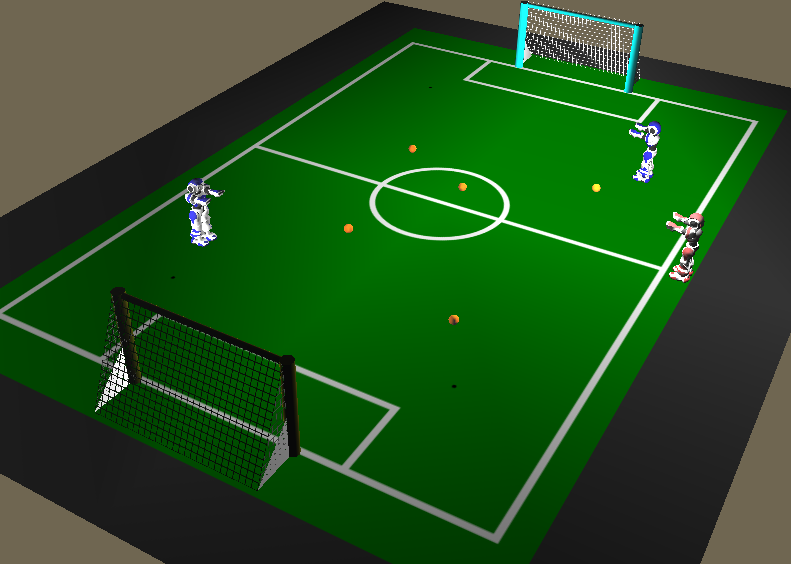
\includegraphics[width=0.75\textwidth]{figures/nao_anyballchallenge.png}
 % nao_anyballchallenge.png: 791x564 pixel, 72dpi, 27.90x19.90 cm, bb=
 \caption{An illustration of an example ``Any ball'' Challenge scenario.}
 \label{fig:anyballchallenge}
\end{figure}

The robot will have 3 minutes to detect the balls, walk towards them, and try to score as many goals as it can. It can kick the ball towards both goals. If the robot is able to score with all balls before the time is over, then the stopwatch will be stopped, time spent for scoring will be recorded, and the team will be awarded with a score of ($180 - \emph{spentTime}$), $180$ being 3 minutes in seconds. The robot will be awarded 20 points for each time it intentionally kicks the balls, and additional 50 points for each goal it scores. An intentional kick is defined as a kick that results in at least 1 meter displacement of the ball. Balls that go inside the goals or out of bounds will be removed. If the robot is not able to score after 3 minutes, then partial credit will be given based on whether the robot showed convincing attempts of detecting, tracking, and kicking the ball. Finally the teams will be ordered based on their scores and their scores will be normalized according to the scoring scheme mentioned in the introduction section.

\section{The Passing Challenge}
\label{sec:passing}
%\newcommand{\passInitMinNum}{15}
%\newcommand{\passMinNum}{two}

This second challenge is similar to the last year's passing challenge of the Humanoid League. It is intended to encourage teams to develop passing and catching skills. In this challenge each team will be required to demonstrate successive passes back and forth between two robots.

The field is marked with two additional white lines, which are parallel to the middle line and tangential to the center circle, as shown in Figure \ref{fig:passingchallenge}. The ball is placed on a penalty kick mark.
One robot is placed inside each penalty area.

\begin{figure}[htbp]
 \centering
 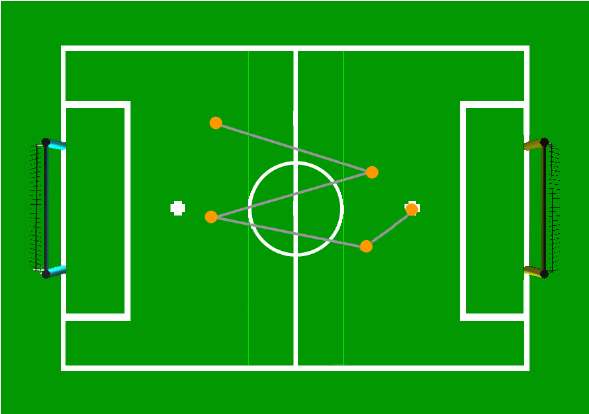
\includegraphics[width=0.75\textwidth]{figures/nao_passingchallenge.png}
 % nao_anyballchallenge.png: 791x564 pixel, 72dpi, 27.90x19.90 cm, bb=
 \caption{Setup and expectations for the Passing Challenge.}
 \label{fig:passingchallenge}
\end{figure}

The robots will have 3 minutes to perform 3 successive passes. The trial ends without success, that is the challenge ends, if the ball or one of the robots leaves the field, or if the ball stops inside the middle area or one of the robots enters the middle area. The ball is expected to cross the middle area 3 times, as indicated by the example trajectory in Figure \ref{fig:passingchallenge}. The trial is considered successful if the receiving robot touches the ball after the third crossing.

Intermediate scoring for passing between robot 1 and 2 (robot 1 is the first kicking one):
\begin{itemize}
 \item $1^{st}$ touch of the ball to robot 2:  1 points
 \item $2^{nd}$ touch of the ball to robot 1:  2 points
 \item $3^{rd}$ touch of the ball to robot 2:  3 points
\end{itemize}

If a team completes the challenge successfully in less than 3 minutes, then the final placement among such teams will be based on how fast the challenge was completed.

\section{The Localization With Obstacle Avoidance Challenge}
\label{sec:localization}

The aim of this challenge is to test the abilities of the robots to get localized on the field and move to their target positions while avoiding the obstacles on the way. This scenario can be thought of as a simulation of the state of the field after a goal is scored, where the robots are mostly on the opposite half of the field and trying to go back to their kick-off positions. 

The TC will pick 3 random points on the field. The coordinate system of the points has its origin at the center point of the field, the +$x$ axis points towards the yellow goal, and the +$y$ axis points to the left. The coordinates will be stored on the USB sticks of the robots by the Technical Committee in the file /media/userdata/points.cfg prior to the challenge\footnote{Please announce early to the TC if this location is not available on the USB stick of your robot}. Here is an example of the file for the positions of the three robots shown in Figure~\ref{fig:anyballchallenge}\footnote{In contrast to the example, the target positions will always be inside the playing area}:
%
{\small\begin{verbatim}
120 -160
-120 160
0 220
\end{verbatim}
}
%
There will also be two blue robots on the field to be used as stationary obstacles. The locations of those robots will be determined randomly at the beginning of the challenge and will be the same for all teams. These obstacles will be at least 50cm away from each of the target points. The starting point of the competing robot will also be determined randomly at the beginning and remain unchanged for all teams. 

The robots are expected to indicate that they think they are on the target points by pausing for 10 seconds and flashing their ear LEDs. When this signal is observed, the referee will pause the stopwatch, place a small marker underneath the center of the robot (approximately the point between the robot's feet), and restart the timer when the robot starts moving. The aim of the robots in this challenge will be to visit those points as fast and accurate as possible.

The trial ends without a success if the robot touches one of the obstacles. If the robot is able to complete the challenge by visiting all three points in less than 3 minutes, then the remaining time will be used to determine the final score of the team. The distances between the visited points and the target points will also be used in the computation of the final score.

When the time is up or the robot stops 3 times as an indication of the belief of arrival, all robot position markers more than 50cm from any target point are disregarded, and if there are multiple markers within 50cm of a single target point then only the closest is kept. Teams are then awarded $150 - d$ points for each visited marker, where $d$ is the distance from the marker to the point in centimeters. They are then awarded $3 \times (180 - t)$ points, where $t$ is the total time used measured in seconds.

Teams will be ranked as follows: First, they will be ranked by the number of markers they reach (within 50cm). When two teams reach the same number of markers, the score determines their rank.

Another way of looking at the scoring is as follows:

\begin{itemize}
 \item You start with 540 points.
 \item You lose 3 points per second.
 \item You get 100 points for reaching a marker (within 50cm). Losing 3 points per second, this means you need to reach that 50cm circle within 33 seconds to make it worth your time.
 \item For each 1cm improvement in accuracy you get another point. Losing 3 points per second, this means you need to increase your accuracy at 3cm/s to make it worth your time. 
\end{itemize}

These scores will be normalized according to the scoring scheme described in the introduction section.

\end{document}


